\chapter{Implementation}
\label{chap:eval}
\section{Imlementation}
The portable probabilistic programming framework is implemented in C and is consisted of four parts: parser, inference engine, query analyzer, and API implementations.

\subsection{Parser}
We implemented the parser based on the grammar in Chapter ~\ref{chap:approach}, Section ~\ref{sec:syntax}. Since the language is used to describe Bayesian networks, we didn't generate abstract syntax tree. Instead, we generate the graph to describe the probabilistic graphical model with the following data structure:
\begin{lstlisting}[language=C]
  struct BNVertex {
    int type;      // draw or compute
    float sample;  // last sampled value
  };
 
  struct BNVertexDraw {
    struct BNVertex super;  // extends BNVertex
    int type;               // dbern, dnorm, dgamma, or constant
  };
 
  struct BNVertexDrawBern {
    struct BNVertexDraw super;
    float p;
  };
 
  struct BNVertexDrawNorm {
    struct BNVertexDraw super;
    float mean;
    float variance;
  };
 
  struct BNVertexDrawGamma {
    struct BNVertexDraw super;
    float a;
    float b;
  };
 
  struct BNVertexDrawConst {
    struct BNVertexDraw super;
    float c;
  };
 
  struct BNVertexCompute {
    struct BNVertex super;  // extends BNVertex
    int type;               // + or if
  };
 
  struct BNVertexComputePlus {
    struct BNVertexCompute super;
    struct BNVertex* left;
    struct BNVertex* right;
  };
 
  struct BNVertexComputeIf {
    struct BNVertexCompute super;
    struct BNVertex* condition;
    struct BNVertex* consequent;
    struct BNVertex* alternative;
  };
\end{lstlisting}
The generated network is (1) constructed, (2) topological sorted, and (3) stored in an array struct \texttt{BNVertex* vertices[]}. The inference engine can traverse this array from the start to the end, and access sample values stored in the vertices. Because the network is already topological sorted, it is guaranteed that inference engine always reads the correct sample values.

\subsection{Probabilistic Distributions}
The implementations of the probabilistic distributions are generally based on rejection sampling. We leveraged the algorithms in probability theory to generate variables from a specified distribution.

Figure ~\ref{fig:gaussian} is an example to show how we derive the samples of Gaussian distribution from \texttt{randomC} distribution which generate random values in $[0, 1]$:

\begin{figure}
\begin{lstlisting}[language=C]
  float gaussian(float mu, float sigma)
  {
      float u, v, x, y, q;
      do {
          u = 1 - randomC();
          v = 1.7156 * (randomC() - 0.5
          x = u - 0.449871;
          y = fabs(v) + 0.386595;
          q = x * x + y * (0.196 * y - 0.25472 * x);
      } while (q >= 0.27597 && (q > 0.27846 || v * v > -4 * u * u * log(u)));
      return mu + sigma * v / u;
  }
\end{lstlisting}
\caption{Sampling Gaussian distribution}
\label{fig:gaussian}
\end{figure}

\subsection{Inference Engine}

\begin{figure}
    \centering
    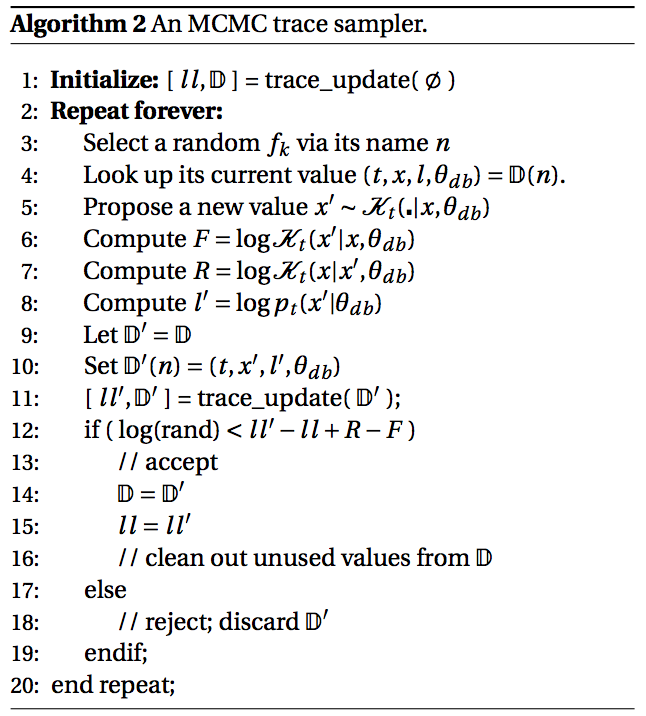
\includegraphics[width=0.7\textwidth]{figures/trace1.png}
    \caption{An MCMC trace sampler.}
    \label{fig:trace1}
\end{figure}

\begin{figure}
    \centering
    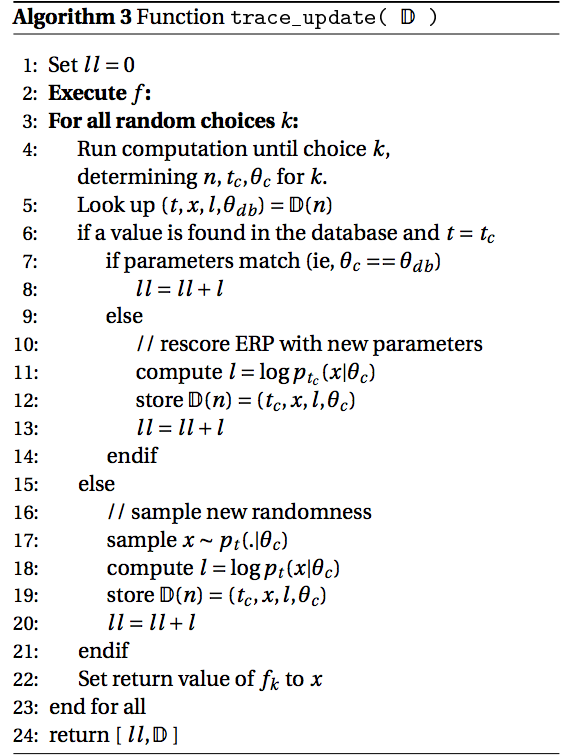
\includegraphics[width=0.7\textwidth]{figures/trace2.png}
    \caption{Algorithm for trace update}
    \label{fig:trace2}
\end{figure}

In the implementation of the MH alorithm in our inference engine, we leverage the approach proposed by ~\cite{lightweight}, which memorized trace information and update trace iteratively. More specifically, Let a database $\mathbb{D}$ be defined as a mapping $ \mathbb{N} \rightarrow \mathscr{T} \times X \times \mathbb{L} \times \theta$, where $\mathbb{N}$ is the name of a random choice, $\mathscr{T}$ is its elementary random primitives(ERP) type, which represents a sample function of distributions like \texttt{rand(), gaussian()}, $X$ is its value, $\theta$ are ERP parameters, and $\mathbb{L}$ is this random value's likelihood. Missing entries are allowed here.

We can control the execution of a function $f'$ by controlling the values in $\mathbb{D}$. When $f'$ encounters an $f_k'$ , it computes its name $n \in \mathbb{N}$, its parameters $\theta_c$ (where $c$ is a mnemonic for ``current"), and its current type $t_c \in \mathscr{T}$. It then looks up $(t,x,l,\theta_{db}) = \mathbb{D}(n)$. If a value is found and the types match, we set the return value of $f_k$ to be $x$. Otherwise, the value is sampled from the appropriate ERP $x \sim p_{t_c}(\cdot|\theta_c)$, its likelihood is computed, and the corresponding entry in the database is updated. This is formalized in the \texttt{trace\_update} procedure, defined in Figure ~\ref{fig:trace2}.

We use \texttt{trace\_update} to define our overall MCMC algorithm, shown in Figure ~\ref{fig:trace1}. Given a current trace $x$ and score $p(x)$, we proceed by reconsidering one random choice $x_k$. We equip each ERP type with a proposal kernel $\mathscr{K}_t(x'|x,\theta)$, which we use to generate proposals to $x_k$. After a proposal, we call \texttt{trace\_update} to generate a new trace $x'$, and compute its likelihood $p(x')$, which is the product of any reused random choices, and any new randomness that was sampled. This gives us an overall score, which is used as an MH accept ratio
\begin{align*}
  \alpha = min \{1, \frac{p(x')\mathscr{K}_t(x|x′,\theta)}{p(x)\mathscr{K}_t(x'|x,\theta)} \}
\end{align*}

There are some other methods to implement an inference engine such as the \textit{nonstandart interpretations} proposed by \cite{nonstandard}, which showed how \textit{nonstandard interpretations} of probabilistic programs can be used to perform efficient inference algorithms. In their method, infromation about the structure of the distributions (which is the dependencies or gradients in the probabilistic graphical models) is derived as monad-like side computation as the same time of executing the program. Meanwhile, the interpretations can be coded easily with some special-purpose objects and operator overloading. They promoted the inference efficiency perfomance by using the structure information of distribution as part of the variety of inference algorithms.

Additionally, because of the program is in a machine-readable form, various of techniques from compiler design and program analysis can be used in the inference engine. ~\cite{gordon2013} designed a new model-learner pattern for Bayesian reasoning. In their work, a new probabilistic programming abstraction was proposed, a typed Bayesian model, based on a pair of probabilistic expressions for the prior and sampling distributions. Also, ~\cite{dataflow} presented a new algorithm for Bayesian inference over probabilistic programs, which is based on data flow analysis techniques from the program analysis community. These can be improvements to our framework in the future development.

\subsection{API}
To enable the APIs for other programming languages, we first compiled the inferface file as showed in Section ~\ref{sec:api} and generated the wrapper code that other languages need to access the underlying C/C++ code. Then the users will have access to the APIs of the portable probabilistic programming language framework in their domain language. 

\section{Case Study}
Following the example we have illustrated above: flip example, which is showed in Figure ~\ref{fig:flip_eg}, we studied the accuracy and time cost according to the different assignments of number of samples. The result is showed in Figure ~\ref{fig:flip_eval1} and Figure  ~\ref{fig:flip_eval2}. 
\begin{figure}
    \centering
    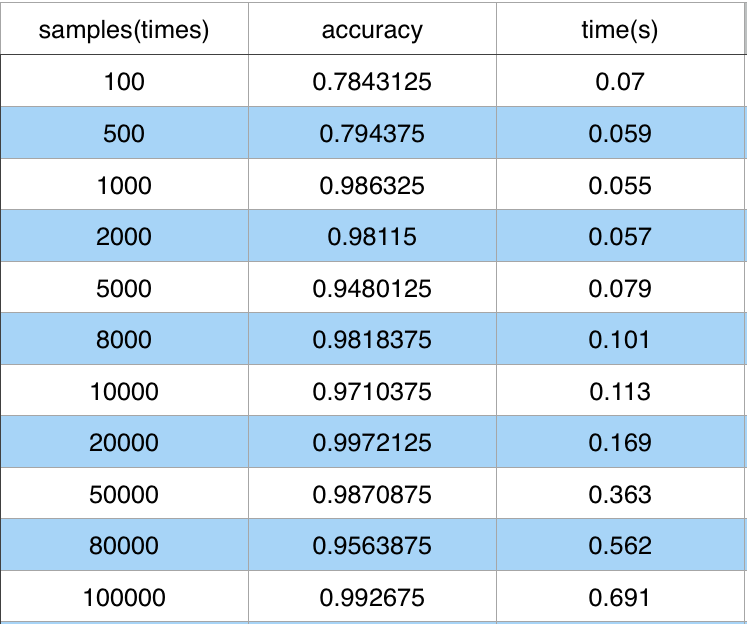
\includegraphics[width=0.7\textwidth]{figures/flip_eval.png}
    \caption{Table of flip example}
    \label{fig:flip_eval1}
\end{figure}

\begin{figure}
    \centering
    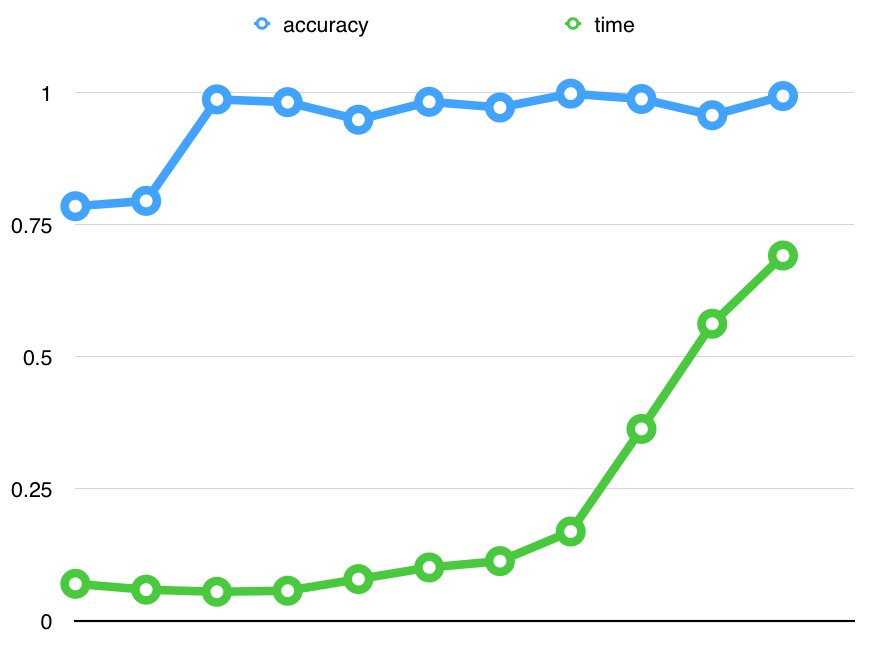
\includegraphics[width=0.7\textwidth]{figures/flip_eval2.png}
    \caption{Flip example: accuracy and time according to the number of samples.}
    \label{fig:flip_eval2}
\end{figure}
